\subsection{The learning activities}
\begin{frame}{Timeline of the students' activities}
    \begin{figure}[tb]
        \begin{center}
            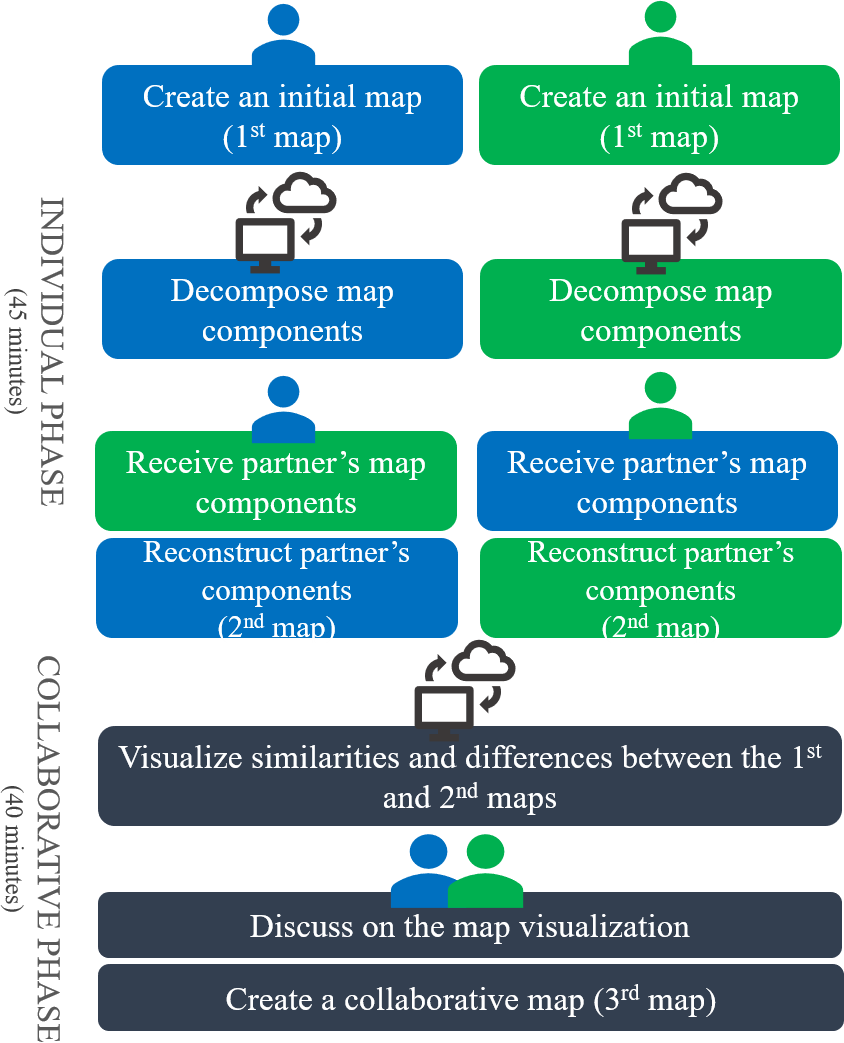
\includegraphics[width=50mm]{images/rqb_learner-activities.pdf}
        \end{center}
    \end{figure}
    {\tiny **Note: Three days after the experiment, the teacher gave feedback to the students. \\
    The consent form to participate and a survey regarding students' affective response
    toward the activities were also collected afterward. }

\end{frame}

\subsection{Participants characteristics}
\begin{frame}{Participants}

\begin{itemize}
    \item <1-> \textcolor{blue}{Forty-four students} of Linear Algebra class
    \item <1-> Majored in \textcolor{blue}{Computer Science or Information System} at a public university in Indonesia
    \item <1> \textcolor{blue}{73\%} of them are \textcolor{blue}{male} students ($n = 32$)
    \item <1> Most of them were the first year students in their second term (ages of 18-22 years old)
    \item <2-> They had \textcolor{blue}{experiences in various collaborative learning} activities
    \item <2-> They were \textcolor{blue}{familiar with concept mapping} and used to create a concept map from scratch
\end{itemize}

\end{frame}

\subsection{Task settings}

\begin{frame}{Selected topic}
\begin{itemize}
    \item Course name: \textcolor{blue}{Linear Algebra} class of 2018
    \item Selected topics: \textcolor{blue}{General Vector Space \& Inner Product Space}
    \item \textcolor{blue}{14} concepts selected as predefined \textcolor{blue}{nodes}
    \item Group formation: \textcolor{blue}{dyad}, selected freely by the students
\end{itemize}

\begin{figure}[tb]
    \begin{center}
            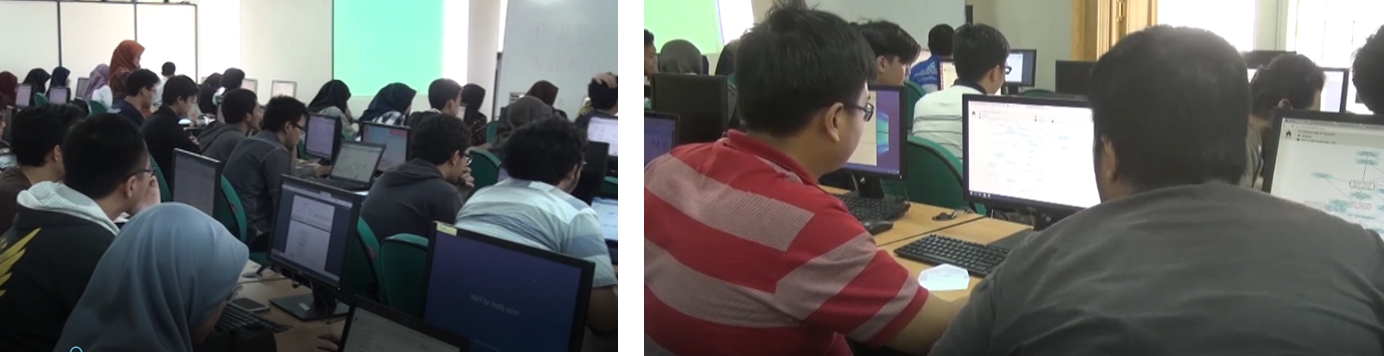
\includegraphics[width=100mm]{images/classroom_situation.png}
        \end{center}
        \caption{Classroom situation}
        \label{intro::classroom}
    \end{figure}
\end{frame}

\begin{frame}{RKB system: Initial user-interface}
    \begin{figure}[tb]
        \begin{center}
            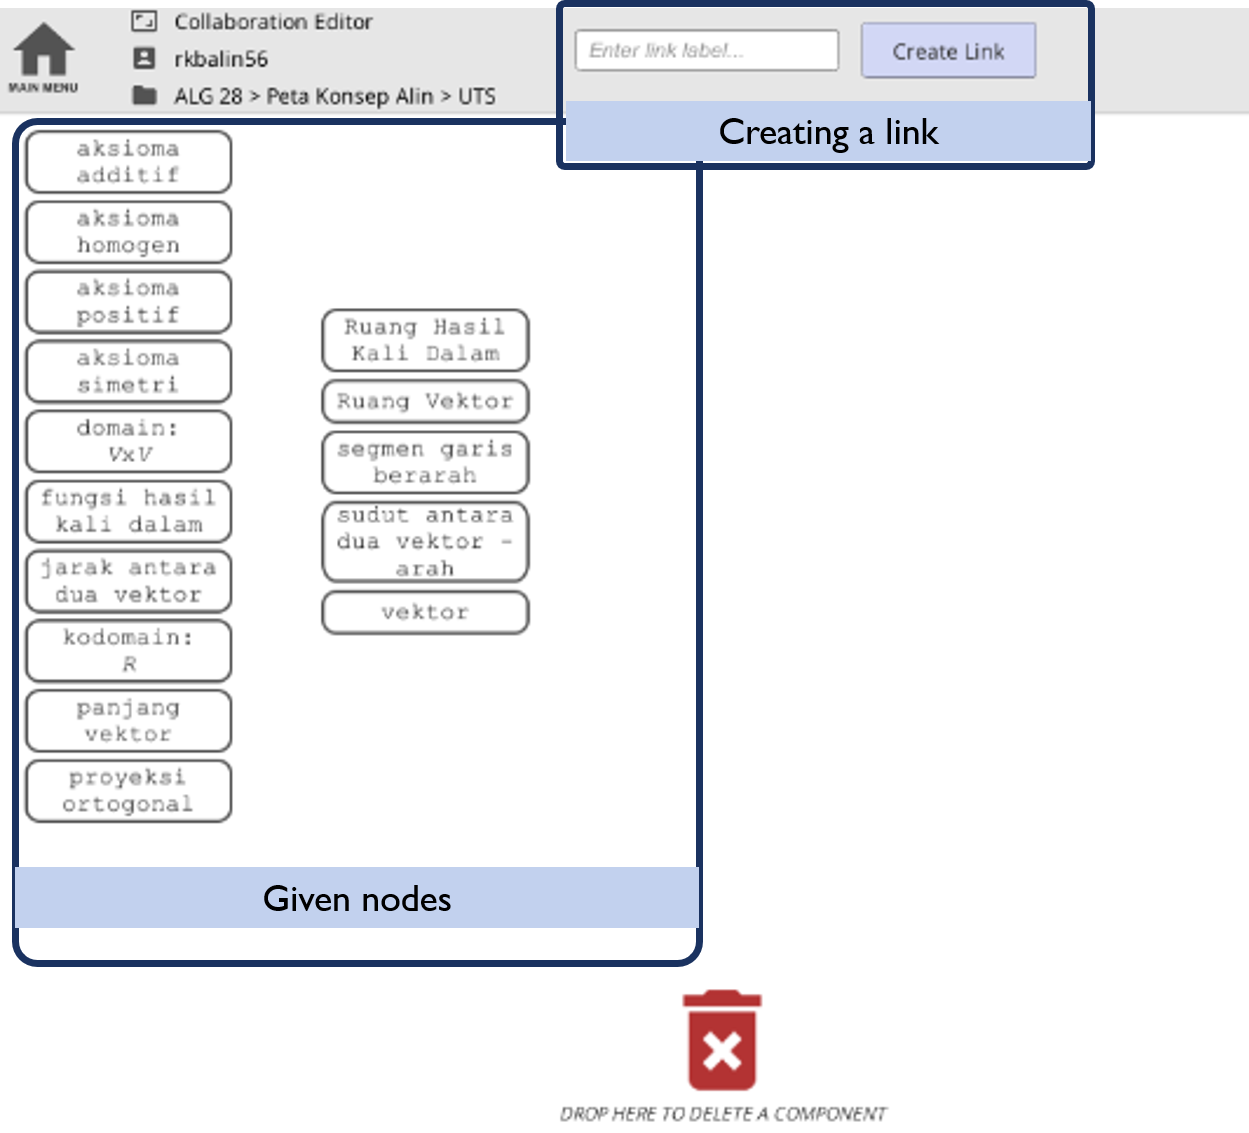
\includegraphics[width=80mm]{images/system_interface.png}
        \end{center}
    \end{figure}
\end{frame}

\begin{frame}{}
    \begin{figure}[tb]
    \begin{center}
        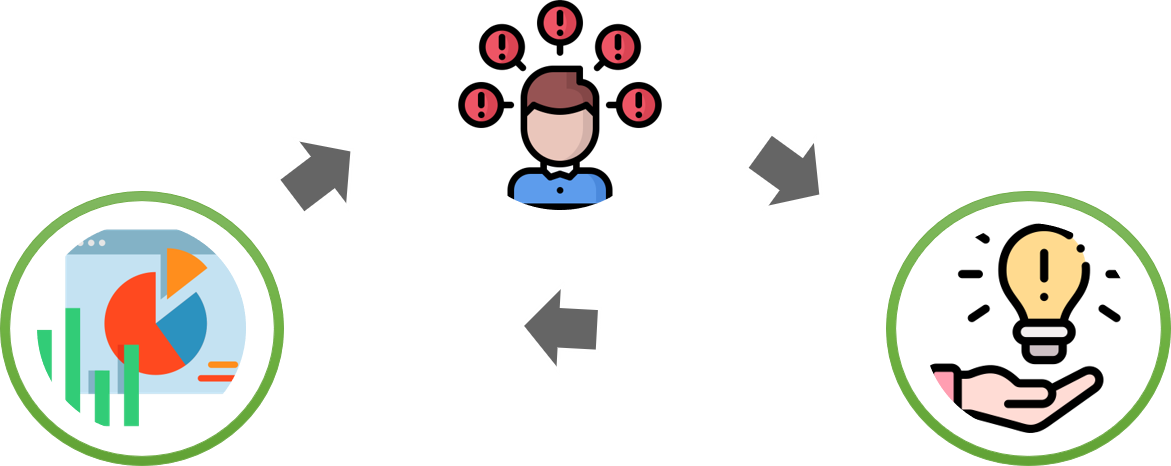
\includegraphics[width=110mm]{images/intro_method_result.png}
    \end{center}
\end{figure}
\end{frame}
\begin{frame}{Research objectives: Revisit}
    Based on the challenges mentioned above, we define the main purposes of this study are as follow: 
    \begin{enumerate}[A]
        \item {\color{blue}to identify the effectiveness of the RKB approach for collaborative concept mapping in a practical classroom};
        \begin{enumerate}
            \item \textcolor{blue}{Collaborative product evaluation
            \item Exploring students' perceptions toward the activity}
        \end{enumerate}
        
        \item to investigate how individual differences in prior knowledge has potentially influence collaborative-learning effectiveness and the students' perceptions toward the activities; 
        %\begin{enumerate}
        %    \item Analyzing the effect of different group formation on collaboration
        %\end{enumerate}
        
        \item to analyze how similarity of individual knowledge and comprehension  of partner's representation could predict the final collaborative products.
        %\begin{enumerate}[4]
        %    \item Predicting group outcomes based on individual maps
        %\end{enumerate}
    \end{enumerate} 
\end{frame}

% \begin{frame}[allowframebreaks]{Reciprocal Kit Build (RKB)}
    
    %\href{run:/path/nameofvideo.mp4}{Click for video}
%      \begin{figure}[tb]
%          \begin{center}
%          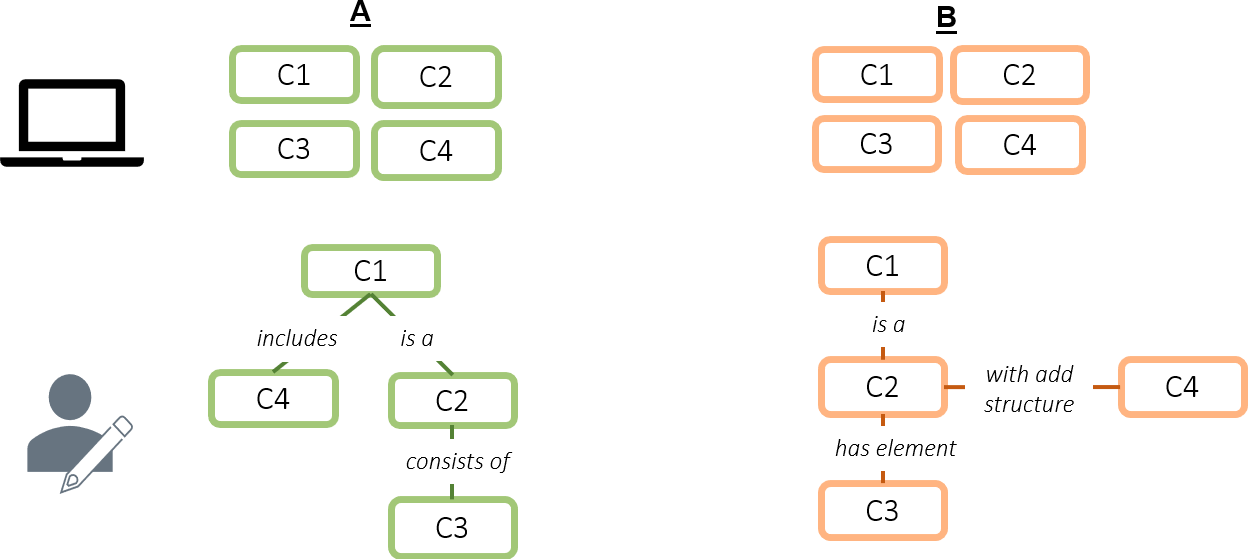
\includegraphics[width=100mm]{images/RKB_p1.pdf}
%          \end{center}
%          \caption{\emph{Individual phase} -- Initial map construction}
%          \label{intro::rkb_p1}
%      \end{figure}
    
%      \begin{figure}[tb]
%          \begin{center}
%              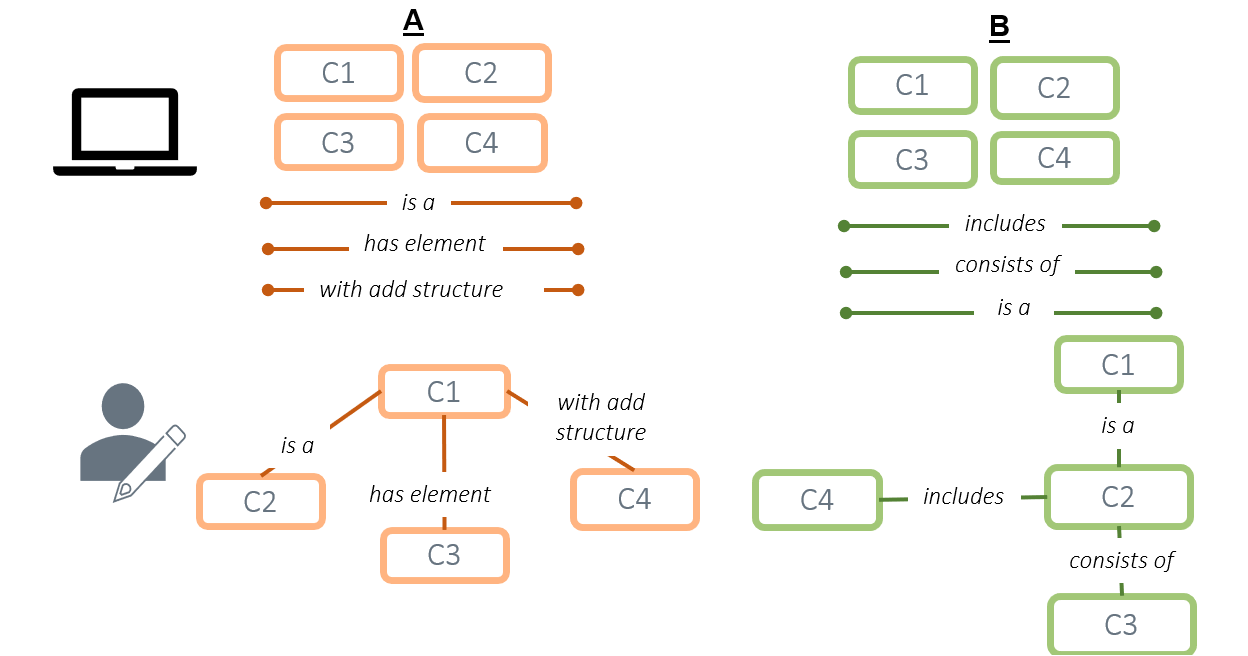
\includegraphics[width=100mm]{images/RKB_p2.pdf}
%          \end{center}
%          \caption{\emph{Individual phase} -- Re-constructional map building}
%          \label{intro::rkb_p2}
%      \end{figure}
    
%     \begin{figure}[tb]
%          \begin{center}
%              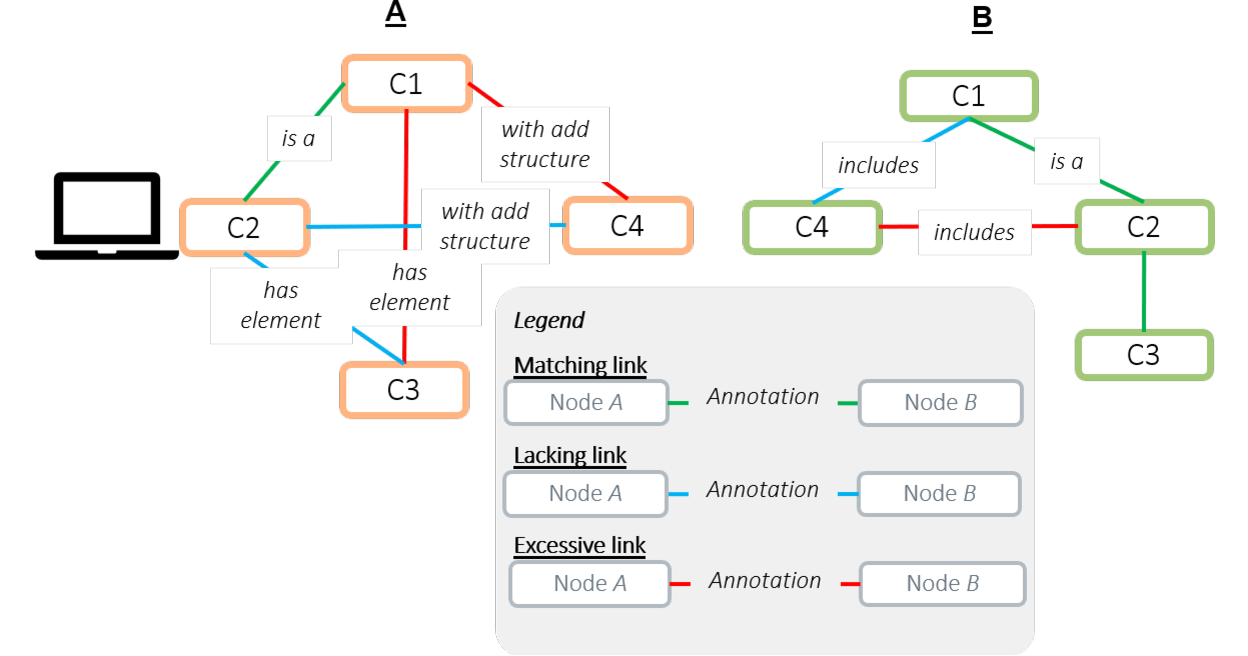
\includegraphics[width=100mm]{images/RKB_p3.pdf}
%          \end{center}
%          \caption{\emph{Collaborative phase} -- Visualization of map similarities and differences \& group discussion}
%          \label{intro::rkb_p3}
%      \end{figure}
    
%      \begin{figure}[tb]
%          \begin{center}
%              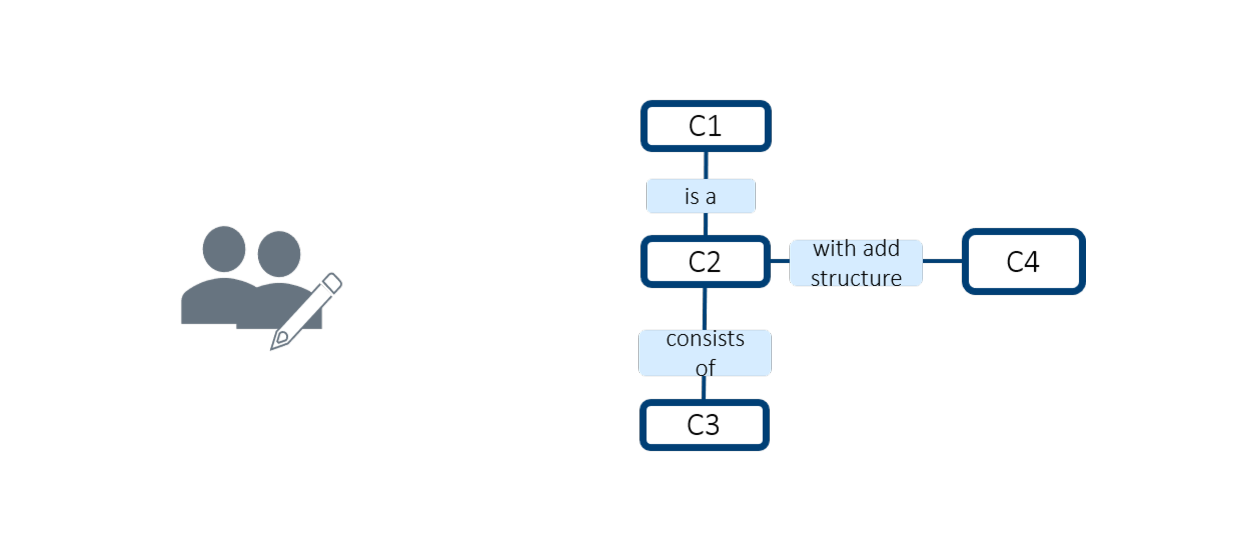
\includegraphics[width=100mm]{images/RKB_p4.pdf}
%          \end{center}
%          \caption{\emph{Collaborative phase} -- Group map construction}
%          \label{intro::rkb_p4}
%      \end{figure}
% \end{frame}


% \begin{frame}{The learning activities during experiment: the individual phase}
%     \begin{figure}[tb]
%         \begin{center}
%             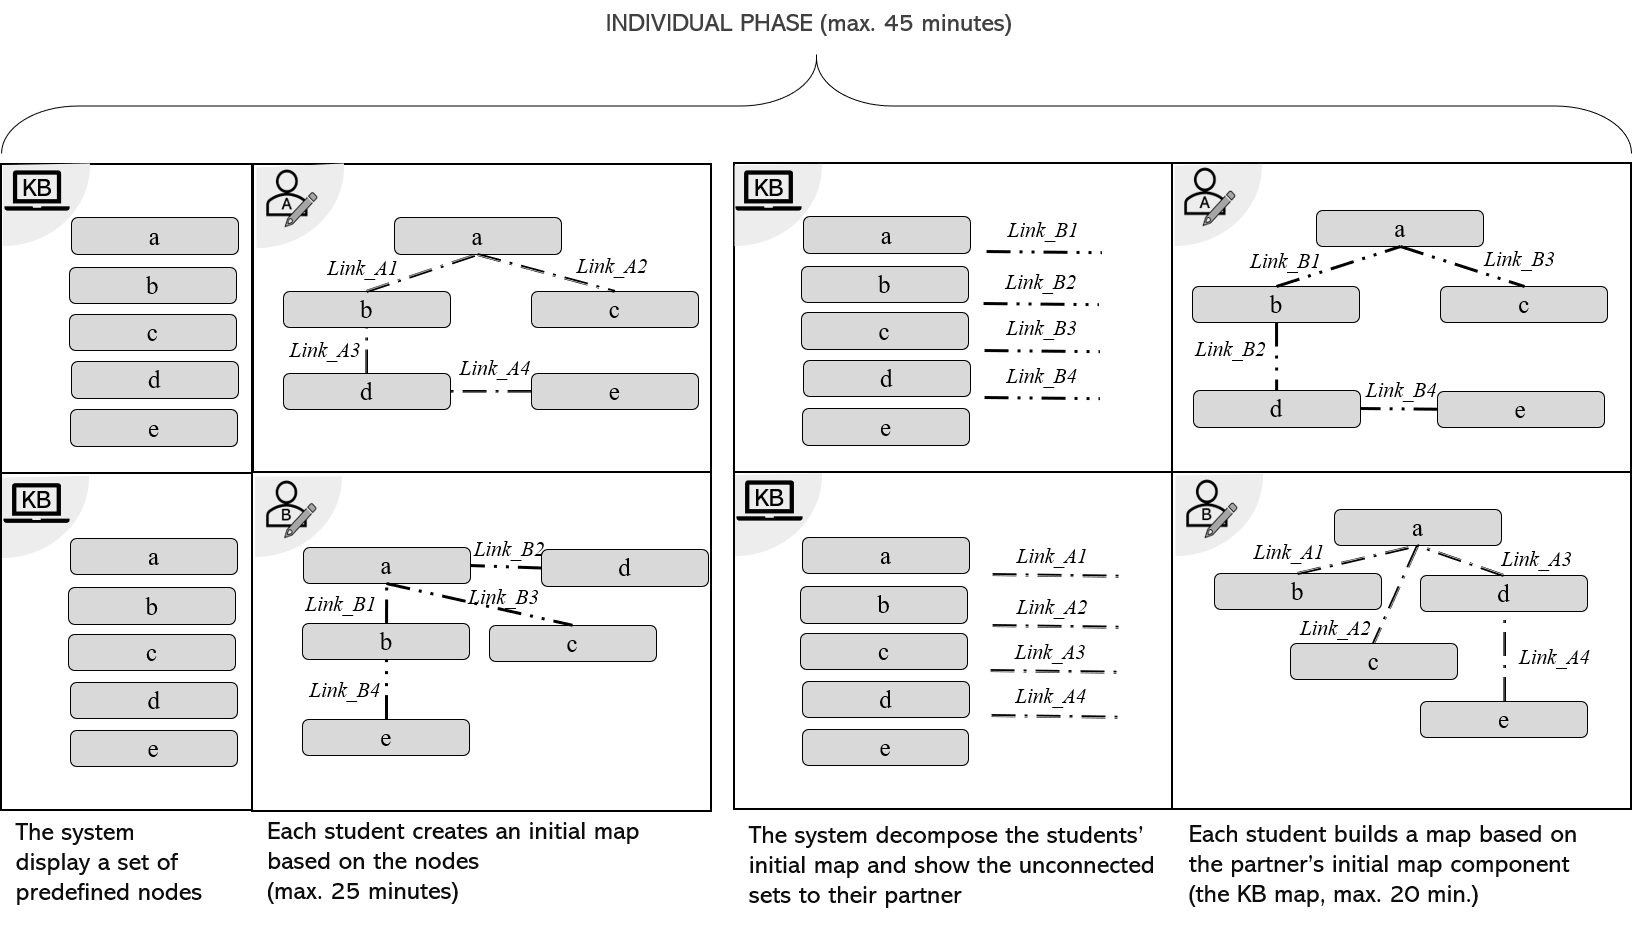
\includegraphics[width=90mm]{images/method_ind_phase_RKB.pdf}
%         \end{center}
%         \caption{Timeline of students' activities (individual phase)}
%         \label{method::rkb_ind_phase}
%     \end{figure}
    
% \end{frame}
% \begin{frame}{The learning activities during experiment: the collaborative phase}
%     \begin{figure}[tb]
%         \begin{center}
%             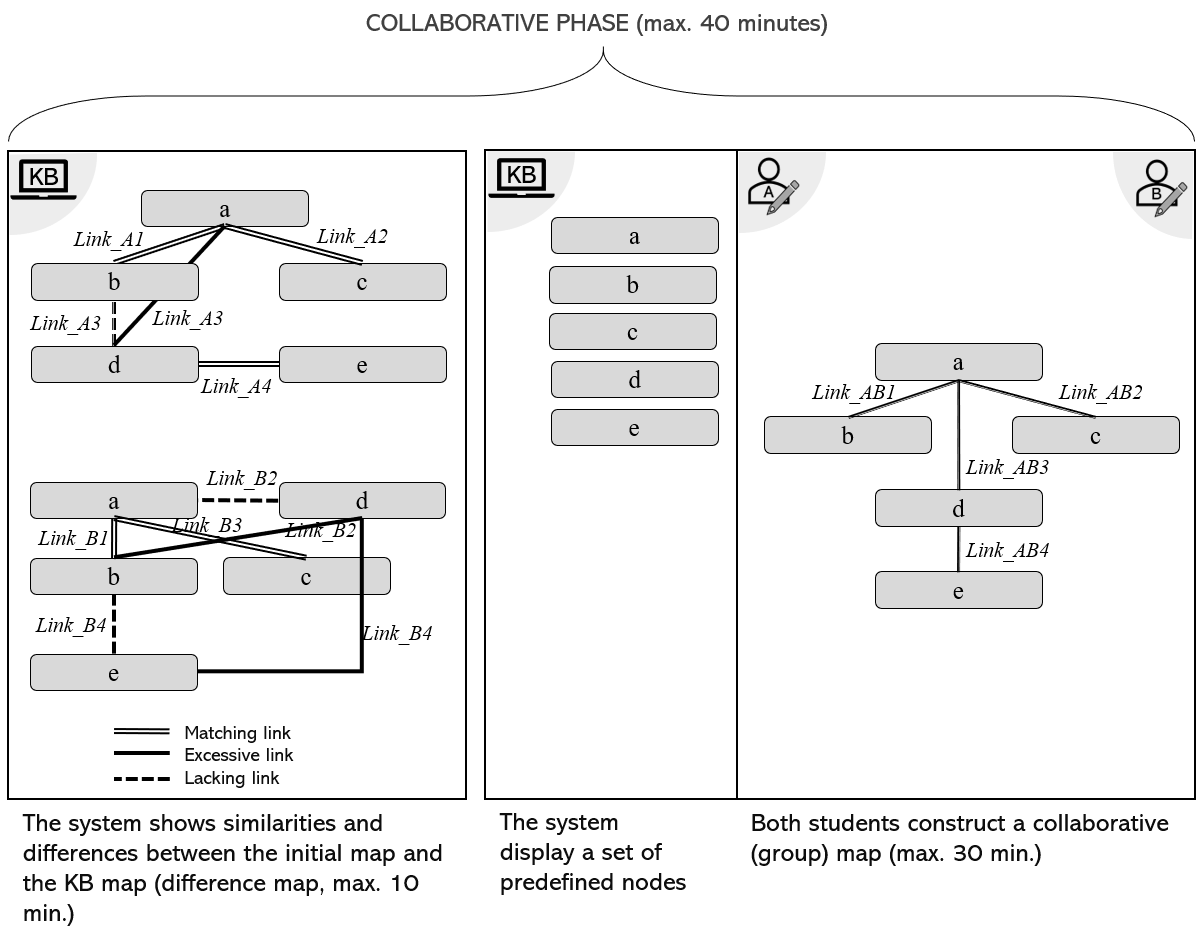
\includegraphics[width=75mm]{images/method_collab_phase_RKB.pdf}
%         \end{center}
%         \caption{Timeline of students' activities (collaborative phase)}
%         \label{intro::rkb_collab_phase}
%     \end{figure}
% \end{frame}
    
    % \begin{table}[tb]
    % \begin{center}
    % \begin{tabular}{p{2.5cm}|p{5.5cm}|p{2cm}}%{c|c|c} %#{ | m{5em} | m{1cm}| m{1cm} | }
    % \hline
    % Phase & Students' Activity & Duration\\
    % \hline
    % Introduction & Kit-Build practice & 5 min.\\
    % Individual & (a) Create a concept map based on the predefined concepts (first map) & 25 min.\\
    % & (b) Create a re-constructional map based on the partner's first map components (second map) & 20 min.\\
    % Collaborative & (a) Discussion on shared and difference maps & 10 min.\\
    % & (b) Create a group concept map  (third map) & 30 min.\\
    % \hline
    % \end{tabular}
    % \end{center}
    % \caption{\label{tab:exp_setting} Timeline of students' activities during experiment}
    % \end{table}
 



